% GNUPLOT: LaTeX picture with Postscript
\begingroup
  \makeatletter
  \providecommand\color[2][]{%
    \GenericError{(gnuplot) \space\space\space\@spaces}{%
      Package color not loaded in conjunction with
      terminal option `colourtext'%
    }{See the gnuplot documentation for explanation.%
    }{Either use 'blacktext' in gnuplot or load the package
      color.sty in LaTeX.}%
    \renewcommand\color[2][]{}%
  }%
  \providecommand\includegraphics[2][]{%
    \GenericError{(gnuplot) \space\space\space\@spaces}{%
      Package graphicx or graphics not loaded%
    }{See the gnuplot documentation for explanation.%
    }{The gnuplot epslatex terminal needs graphicx.sty or graphics.sty.}%
    \renewcommand\includegraphics[2][]{}%
  }%
  \providecommand\rotatebox[2]{#2}%
  \@ifundefined{ifGPcolor}{%
    \newif\ifGPcolor
    \GPcolortrue
  }{}%
  \@ifundefined{ifGPblacktext}{%
    \newif\ifGPblacktext
    \GPblacktexttrue
  }{}%
  % define a \g@addto@macro without @ in the name:
  \let\gplgaddtomacro\g@addto@macro
  % define empty templates for all commands taking text:
  \gdef\gplbacktext{}%
  \gdef\gplfronttext{}%
  \makeatother
  \ifGPblacktext
    % no textcolor at all
    \def\colorrgb#1{}%
    \def\colorgray#1{}%
  \else
    % gray or color?
    \ifGPcolor
      \def\colorrgb#1{\color[rgb]{#1}}%
      \def\colorgray#1{\color[gray]{#1}}%
      \expandafter\def\csname LTw\endcsname{\color{white}}%
      \expandafter\def\csname LTb\endcsname{\color{black}}%
      \expandafter\def\csname LTa\endcsname{\color{black}}%
      \expandafter\def\csname LT0\endcsname{\color[rgb]{1,0,0}}%
      \expandafter\def\csname LT1\endcsname{\color[rgb]{0,1,0}}%
      \expandafter\def\csname LT2\endcsname{\color[rgb]{0,0,1}}%
      \expandafter\def\csname LT3\endcsname{\color[rgb]{1,0,1}}%
      \expandafter\def\csname LT4\endcsname{\color[rgb]{0,1,1}}%
      \expandafter\def\csname LT5\endcsname{\color[rgb]{1,1,0}}%
      \expandafter\def\csname LT6\endcsname{\color[rgb]{0,0,0}}%
      \expandafter\def\csname LT7\endcsname{\color[rgb]{1,0.3,0}}%
      \expandafter\def\csname LT8\endcsname{\color[rgb]{0.5,0.5,0.5}}%
    \else
      % gray
      \def\colorrgb#1{\color{black}}%
      \def\colorgray#1{\color[gray]{#1}}%
      \expandafter\def\csname LTw\endcsname{\color{white}}%
      \expandafter\def\csname LTb\endcsname{\color{black}}%
      \expandafter\def\csname LTa\endcsname{\color{black}}%
      \expandafter\def\csname LT0\endcsname{\color{black}}%
      \expandafter\def\csname LT1\endcsname{\color{black}}%
      \expandafter\def\csname LT2\endcsname{\color{black}}%
      \expandafter\def\csname LT3\endcsname{\color{black}}%
      \expandafter\def\csname LT4\endcsname{\color{black}}%
      \expandafter\def\csname LT5\endcsname{\color{black}}%
      \expandafter\def\csname LT6\endcsname{\color{black}}%
      \expandafter\def\csname LT7\endcsname{\color{black}}%
      \expandafter\def\csname LT8\endcsname{\color{black}}%
    \fi
  \fi
    \setlength{\unitlength}{0.0500bp}%
    \ifx\gptboxheight\undefined%
      \newlength{\gptboxheight}%
      \newlength{\gptboxwidth}%
      \newsavebox{\gptboxtext}%
    \fi%
    \setlength{\fboxrule}{0.5pt}%
    \setlength{\fboxsep}{1pt}%
    \definecolor{tbcol}{rgb}{1,1,1}%
\begin{picture}(7200.00,4740.00)%
    \gplgaddtomacro\gplbacktext{%
    }%
    \gplgaddtomacro\gplfronttext{%
      \csname LTb\endcsname%%
      \put(161,2377){\rotatebox{-270}{\makebox(0,0){\strut{}ylabel $x$}}}%
      \csname LTb\endcsname%%
      \put(3849,123){\makebox(0,0){\strut{}xlabel $f(x)$ }}%
      \csname LTb\endcsname%%
      \put(3911,4033){\makebox(0,0)[r]{\strut{}$n=0$}}%
      \csname LTb\endcsname%%
      \put(3911,3858){\makebox(0,0)[r]{\strut{}$n=1$}}%
      \csname LTb\endcsname%%
      \put(3911,3682){\makebox(0,0)[r]{\strut{}$n=2$}}%
      \csname LTb\endcsname%%
      \put(3911,3506){\makebox(0,0)[r]{\strut{}$n=3$}}%
      \csname LTb\endcsname%%
      \put(3911,3330){\makebox(0,0)[r]{\strut{}\footnotesize $sin(x)$}}%
      \csname LTb\endcsname%%
      \put(714,562){\makebox(0,0)[r]{\strut{}$-1.5$}}%
      \csname LTb\endcsname%%
      \put(714,1167){\makebox(0,0)[r]{\strut{}$-1$}}%
      \csname LTb\endcsname%%
      \put(714,1772){\makebox(0,0)[r]{\strut{}$-0.5$}}%
      \csname LTb\endcsname%%
      \put(714,2377){\makebox(0,0)[r]{\strut{}$0$}}%
      \csname LTb\endcsname%%
      \put(714,2982){\makebox(0,0)[r]{\strut{}$0.5$}}%
      \csname LTb\endcsname%%
      \put(714,3587){\makebox(0,0)[r]{\strut{}$1$}}%
      \csname LTb\endcsname%%
      \put(714,4192){\makebox(0,0)[r]{\strut{}$1.5$}}%
      \csname LTb\endcsname%%
      \put(1338,386){\makebox(0,0){\strut{}$-\pi$}}%
      \csname LTb\endcsname%%
      \put(2593,386){\makebox(0,0){\strut{}$-\pi/2$}}%
      \csname LTb\endcsname%%
      \put(3849,386){\makebox(0,0){\strut{}$0$}}%
      \csname LTb\endcsname%%
      \put(5104,386){\makebox(0,0){\strut{}$\pi/2$}}%
      \csname LTb\endcsname%%
      \put(6360,386){\makebox(0,0){\strut{}$\pi$}}%
      \csname LTb\endcsname%%
      \put(4578,1288){\makebox(0,0){\strut{}\begin{minipage}[c]{\textwidth}\begin{equation*}\sin(x) = \sum_0^{+\infty} \frac{(-1)^n}{(2n + 1)!} x^{2n+1}\end{equation*} \end{minipage}}}%
      \csname LTb\endcsname%%
      \put(3849,4456){\makebox(0,0){\strut{}Title: Polynomial approximation of sin(x)}}%
    }%
    \gplbacktext
    \put(0,0){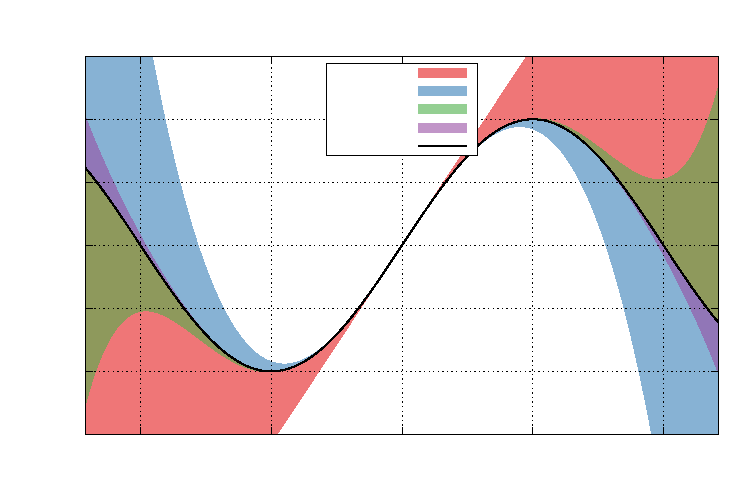
\includegraphics[width={360.00bp},height={237.00bp}]{test}}%
    \gplfronttext
  \end{picture}%
\endgroup
